\documentclass[12pt]{article}
\usepackage[T2A]{fontenc}
\usepackage[utf8]{inputenc}
\usepackage{multirow}
\usepackage{caption}
\usepackage{subcaption}
\usepackage{amsmath}
\usepackage{changepage}
\usepackage{graphicx}
\usepackage{float}
\usepackage[english,russian]{babel}
\usepackage{amsmath, amsfonts, amssymb, amsthm, mathtools}
\usepackage{xcolor}
\usepackage{array}
\usepackage{hyperref}
\usepackage[top = 1.5cm, left = 1.5 cm, right = 1.5 cm, bottom = 3 cm]{geometry}
\graphicspath{ {./images/} }
 
\title{Измерение ускорения свободного падения с использованием физического маятника}
\author{Шахматов Андрей, Б02-304}
\date{\today}
  
\begin{document}
\begin{titlepage}
    \begin{center}
        {\large МОСКОВСКИЙ ФИЗИКО-ТЕХНИЧЕСКИЙ ИНСТИТУТ (НАЦИОНАЛЬНЫЙ ИССЛЕДОВАТЕЛЬСКИЙ УНИВЕРСИТЕТ)}
    \end{center}
    \begin{center}
        {\large Физтех-школа физики и исследований им. Ландау}
    \end{center}
    
    
    \vspace{3cm}
    {\huge
        \begin{center}
            \textbf{Измерение ускорения свободного падения с использованием физического маятника}
        \end{center}
    }
    \vspace{2cm}
    \begin{flushright}
        {\LARGE Автор:\\ Шахматов Андрей Юрьевич \\
            \vspace{0.2cm}
            Б02-304}
    \end{flushright}
    \vspace{7 cm}
    \begin{center}
        Долгопрудный 2023
    \end{center}
\end{titlepage}

% \maketitle

\begin{abstract}
    При помощи метода, основанном на измерении периода колебаний физического маятника, определено значение ускорения свободного падения на географических
    координатах ($55^\circ$ с. ш. $37^\circ$ в. д). Получено значение ускорения свободного падения $g = 9.49 \frac{\textrm{м}}{\textrm{c}^2}$ с 
    относительной погрешностью $0.6\%$. Произведено сравнение экспериментального значения ускорения свободного падения с теоретическим.

\end{abstract}

\tableofcontents

\section{Введение}

Точное измерение ускорения свободного падения является важной задачей геологии. Используя полученное значение, можно провести геологическую
разведку и определить наличие полезных ископаемых в толще земной коры. Самыми доступными методами измерения свободного падения являются методы,
основанные на использовании маятника, пружинных весов или свободно падающего тела. Метод измерения, основанный на использовании пружинных весов,
требует точного определения коэффициента жёсткости пружины, а также учёта нелинейности сжатия пружины. Метод, использующий свободно падающее
тело требует точного детектора, определяющего положение тела, а также проведения измерений в вакууме. Метод, использующий маятник, оказывается 
самым доступным из предложенных, однако также имеет недостатки, такие как необходимость расчёта момента инерции и центра масс маятника, а также нелинейное 
поведение при больших амплитудах. Цель настоящей работы заключалась определении ускорения свободного падения с использованием физического маятника.

\section{Методика}
\subsection{Период колебаний произвольного физического маятника}
Для произвольного физического маятника (Рис. \ref{fig:1}) с моментом инерции $J_0$ относительно оси, проходящей через точку подвеса $O$
параллельно плоскости колебаний, и расстоянием от точки подвеса до центра масс $l$, и массой $M$ справедливо выражение:
\begin{equation}\label{eq:1}
    J_0\ddot{\alpha} = -Mgl\sin{\alpha}.
\end{equation}
Для амплитуд $\alpha \ll 1$ можно приближённо записать:
\begin{equation}\label{eq:2}
    J_0\ddot{\alpha} + Mgl\alpha = 0.
\end{equation}
Выражение \ref{eq:2} является уравнением гармонических колебаний с периодом $T = 2\pi\sqrt{\frac{J_0}{Mgl}}$.

\begin{figure}
    \begin{center}
        \includegraphics[width=0.4\textwidth]{ph1}
    \end{center}
    \caption{Произвольный физический маятник}
    \label{fig:1}
\end{figure}

\subsection{Измерение ускорения свободного падения}
Для проведения эксперимента использовался маятник, который представляет собой длинный однородный стержень, прикреплённый к точке подвеса
при помощи металлической призмы. Изменение момента инерции маятника происходит за счёт подвешивания к разным точкам стержня цилиндрического
груза. Количество колебаний и время колебаний рассчитывается специальным счётчиком. Измерение всех длин производится штангенциркулем. Измерение
массы всех компонентов производится при помощи весов. Погрешности всех измерительных приборов приведены в приложении \ref{sec:app_1}.

% Для проведения эксперимента использовался маятник (Рис. \ref{fig:2}), который представляет собой длинный однородный стержень, прикреплённый к точке подвеса
% при помощи металлической призмы. Изменение момента инерции маятника происходит за счёт подвешивания к разным точкам стержня цилиндрического
% груза. Количество колебаний и время колебаний рассчитывается специальным счётчиком. Измерение всех длин производится штангенциркулем. Измерение
% массы всех компонентов производится при помощи весов. Погрешности всех измерительных приборов приведены в приложении \ref{sec:app_1}.

% \begin{figure}[H]
%     \begin{center}
%         \includegraphics[width=0.4\textwidth]{ph2}
%     \end{center}
%     \caption{Установка, использованная в эксперименте}
%     \label{fig:2}
% \end{figure}

Первоначально определим амплитуду колебаний, при котором погрешность, связанная с нелинейностью колебаний меньше, чем приборная погрешность.
Для этого измерим период колебаний $T_1$ с амплитудой $\alpha_1$, если разность $T_1$ с последующим измерением $T_2$ при амплитуде $\alpha_2$
будет сравнима с приборной погрешностью, то можно считать, что амплитуда $\alpha_2 \ll 1$.

Общий момент инерции $J_0$ рассчитывается как сумма моментов инерции призмы, стержня и груза (Прил. \ref{sec:app_2}). Общий момент
сил рассчитывается по формуле:
\begin{equation}\label{eq:4}
    F = -(Mgl + mgx - {m_p}ga)\sin{\alpha}
\end{equation}
Получим выражение для периода колебаний маятника $T$:
\begin{equation}\label{eq:8}
    T = 2\pi\sqrt{\frac{J + J_p + J_m + mx^2}{Mgl + mgx - {m_p}ga}}
\end{equation}
Положение центра масс призмы $a$ и значение её момента инерции $J_p$ невозможно измерить доступными способами, исключим один из параметров
используя построение графика. После получения экспериментальных данных оценим вклад $a$ и $J_p$ и выберем координатные оси для построения 
графика.

\section{Результаты и их анализ}
Измерены периоды колебаний маятника без груза при начальных амплитудах $10^\circ$ и $5^\circ$, каждое измерение представляет измерение 100
колебаний:
$$T_{10} = 1.5328 \textrm{ c}$$
$$T_5 = 1.5324 \textrm{ c}$$
Приборная погрешность равна $0.1 \textrm{ мc}$, что сравнимо с $T_{10} - T_{5} = 0.4 \textrm{ мc} \thicksim 0.1 \textrm{ мc}$. Значит, что при
начальной амплитуде $5^\circ$ можно считать колебания линейными, а погрешность $T$: 
$$\sigma_T = \sqrt{(T_{10} - T_{5})^2 + 0.1^2} \approx 0.5 \textrm{ мc}$$

Массы стрежня, груза и призмы представлены в таблице \ref{tab:1}, приложение \ref{sec:app_3}. Расстояние до центра масс призмы оценим в $1.5$ см.
Используя формулы \ref{eq:5}, \ref{eq:6}, \ref{eq:7}, рассчитаны моменты инерции компонентов маятника:
$$J = (0.1546 \pm 0.0001)\textrm{ кг}\cdot\textrm{м}^2$$
$$J_m = 6.63 \cdot 10^{-5}\textrm{ кг}\cdot\textrm{м}^2$$
$$J_p \approx 3.12 \cdot 10^{-5}\textrm{ кг}\cdot\textrm{м}^2$$
Значения моментов инерции $J_m$ и $J_p$ сопоставимы с приборной погрешностью $J$, потому можно пренебречь их вкладом в формулу \ref{eq:8}
и пересчитать погрешность для $J$:
$${\sigma_J}' = \sqrt{{\sigma_J}^2 + {J_m}^2 + {J_p}^2} = 0.0002 \textrm{ кг}\cdot\textrm{м}^2$$
Формула \ref{eq:8} примет вид:
\begin{equation}\label{eq:11}
    T = 2\pi\sqrt{\frac{J + mx^2}{Mgl + mgx - {m_p}ga}}
\end{equation}
Тогда используем линеаризацию:
\begin{equation}\label{eq:12}
    \Bigg[\frac{4\pi^2}{T^2}(\frac{J}{m} + x^2)\Bigg](x) = gx + \frac{Mgl - {m_p}ga}{m}
\end{equation}
График зависимости $Q = \frac{4\pi^2}{T^2}(\frac{J}{m} + x^2)$ от $x$ представлен на рисунке \ref{fig:3}. Данные зависимости представлены
в приложении \ref{sec:app_4} в таблице \ref{tab:2}.
\begin{figure}[H]
    \begin{center}
        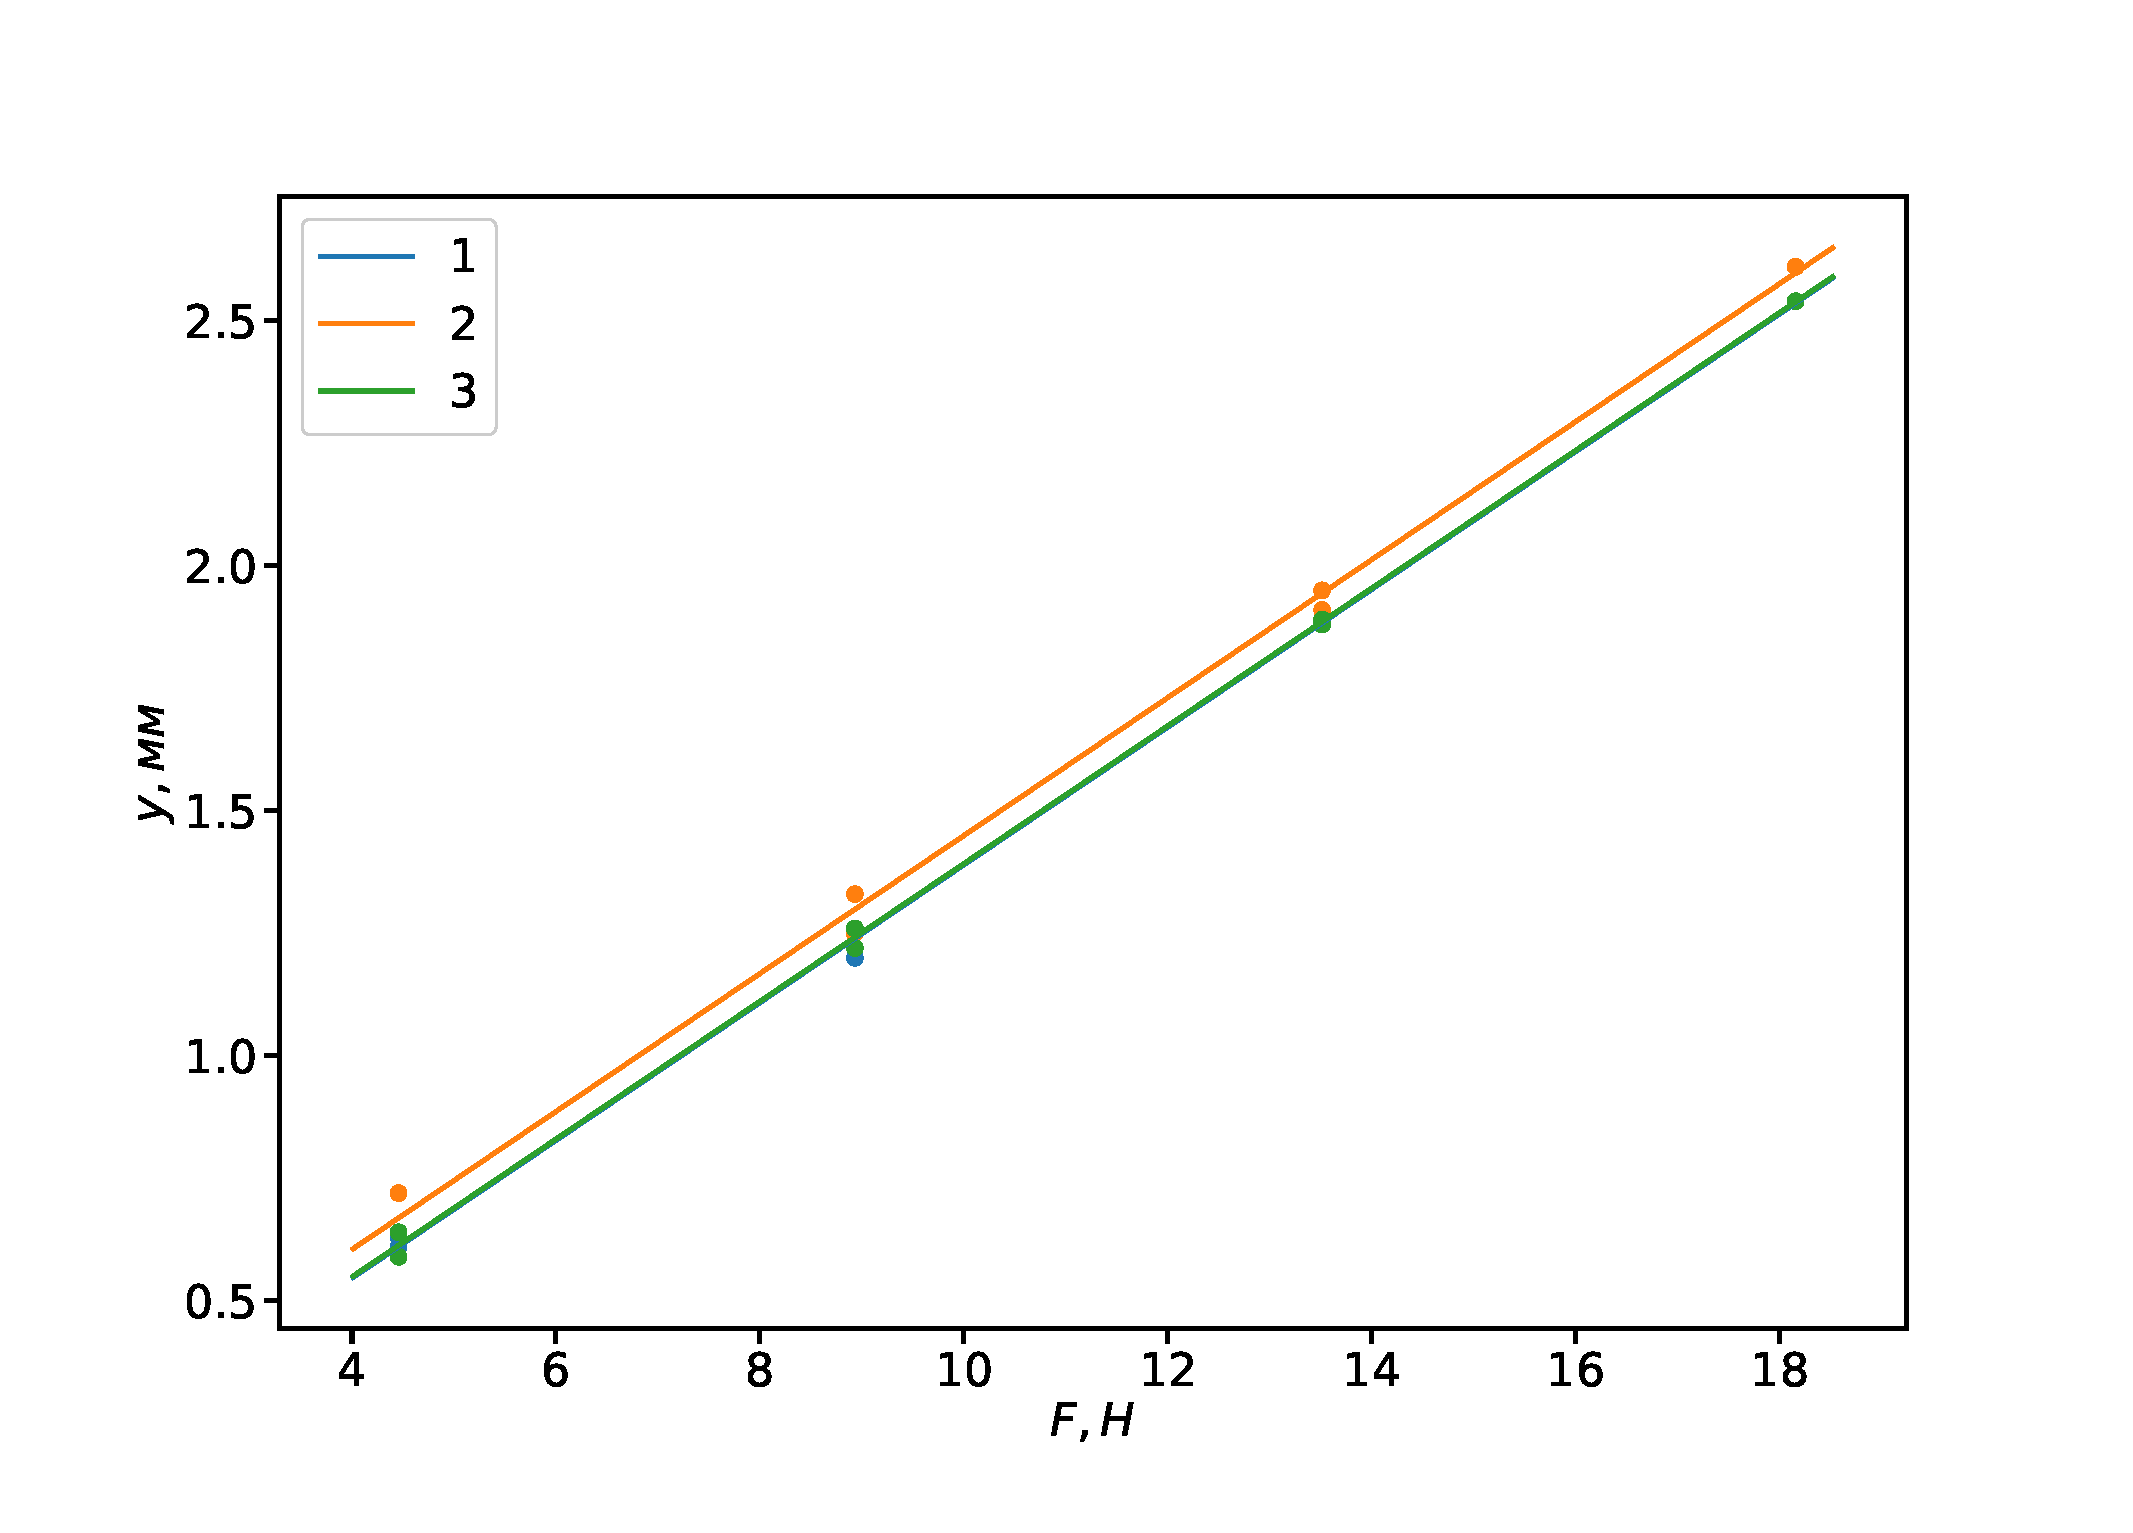
\includegraphics[width=0.8\textwidth]{gr1.eps}
    \end{center}
    \caption{График зависимости $Q = \frac{4\pi^2}{T^2}(\frac{J}{m} + x^2)$ от $x$. Максимальная погрешность по оси $x$ равна 
    $0.1 \textrm{ мм}$, что много меньше масштаба графика по оси x, потому кресты погрешностей по оси x не были нанесены. Максимальная погрешность по
    оси $Q$ равна $0.03 \frac{\textrm{м}^2}{\textrm{с}^2}$ (Прил. \ref{sec:app_5}), что много меньше масштаба графика по оси $Q$, потому кресты
    погрешностей по оси $Q$ не были нанесены.}
    \label{fig:3}
\end{figure}
Из графика следует, что полученная зависимость может быть аппроксимирована прямой, а значит использованная модель маятника корректна.
Коэффициент наклона графика численно равен ускорению свободного падения (Формула \ref{eq:12}). Рассчитано значение $g$ ускорения свободного
падения:
$$g = 9.49 \frac{\textrm{м}}{\textrm{c}^2}$$
Погрешность полученного значения складывается из случайной и приборной погрешности и равна (Прил. \ref{sec:app_5}):
$$\sigma_g = 0.05 \frac{\textrm{м}}{\textrm{c}^2}$$
Итоговая величина ускорения свободного падения равна $g = (9.49 \pm 0.05) \frac{\textrm{м}}{\textrm{c}^2}$, относительная погрешность результата
составляет $0.6\%$.
Полученное значение ускорения свободного падения не совпадает с общепринятым $g = 9.81 \frac{\textrm{м}}{\textrm{c}^2}$,
такое расхождение может объясняться неучтённой систематической ошибкой измерения, связанной с наличием силы сопротивления воздуха, либо
недостаточным количеством повторений измерения периода.

\section{Выводы}
Найден метод измерения ускорения свободного падения, обеспечивающий точность измерения $0.5\%$. Значение ускорения свободного падения,
измеренное данным способом, оказалось равно $g = (9.49 \pm 0.05) \frac{\textrm{м}}{\textrm{c}^2}$. Полученное значение не совпало с 
общепринятым $9.81 \frac{\textrm{м}}{\textrm{c}^2}$, что может быть связано с наличием систематической ошибки или недостаточным количеством
измерений.

\section{Использованная литература}
\begin{thebibliography}{9}
    \bibitem{LabBook}
    Лабораторный практикум по общей физике, Том 1, под редакцией А. Д. Гладуна
\end{thebibliography}

\section{Приложения}
\subsection{Погрешности измерительных приборов} \label{sec:app_1}
Погрешность штангенциркуля - 0.1 мм\\
Погрешность весов - 0.5 г\\
Погрешность секундомера - 10 мс.

\subsection{Моменты инерции составляющих маятника} \label{sec:app_2}
Момент инерции стержня $J$ находится по теореме Гюйгенса-Штейнера:
\begin{equation}\label{eq:5}
    J = \frac{ML^2}{12} + Ml^2
\end{equation}
Момент инерции найден в приближении формы груза цилиндрической с высотой $h$, внутренним и внешним радиусами $r_1$ и $r_2$:
$$J_m = \frac{1}{12}m[3(r_1^2 + r_2^2) + h^2]$$
Тогда полный момент инерции груза в соответствии с теоремой Гюйгенса-Штейнера:
\begin{equation}\label{eq:6}
    J_g = J_m + mx^2
\end{equation}

Момент инерции призмы невозможно вычислить, однако возможно оценить:
\begin{equation}\label{eq:7}
    J_p \approx {m_p}a^2
\end{equation}

Погрешности $J$ и $J_m$ рассчитываются по формулам:
\begin{equation}\label{eq:9}
    \sigma_J = \sqrt{(\frac{ML}{6}\sigma_L)^2 + (2Ml\sigma_l)^2 + ([\frac{L^2}{12} + l^2]\sigma_M)^2}
\end{equation}
\begin{equation}\label{eq:10}
    \sigma_{J_m} = \sqrt{(\frac{r_2}{2}m\sigma_{r_2})^2 + (\frac{r_1}{2}m\sigma_{r_1})^2 +
        (\frac{h}{6}m\sigma_h)^2 + (\frac{1}{12}[3(r_1^2 + r_2^2) + h^2]\sigma_m)^2}
\end{equation}

\subsection{Параметры компонентов маятника} \label{sec:app_3}
\begin{table}[H]
    \begin{center}
        \begin{tabular}{|l|l|l|l|}
            \hline
            $M$, г           & $m$, г          & $m_p$, г       & $L$, см           \\
            \hline
            891.9 $\pm$ 0.5  & 291.0 $\pm$ 0.5 & 78.2 $\pm$ 0.5 & 100.00 $\pm$ 0.01 \\
            \hline
            \hline
            $l$, см          & $h$, см         & $r_1$, см      & $r_2$ , см        \\
            \hline
            30.00 $\pm$ 0.01 & 1.66 $\pm$ 0.01 & 0.60 $\pm$ 0.01 & 2.80 $\pm$ 0.01    \\
            \hline
        \end{tabular}
    \end{center}
    \caption{Параметры компонентов маятника. $M$ - масса стержня, $m$ - масса груза, $m_p$ - масса призмы,
        $L$ - длина стержня, $l$ - длина от точки подвеса до центра масс, $h$ - толщина груза, $r_1$ - внутренний радиус груза,
        $r_2$ - внешний радиус груза.}
    \label{tab:1}
\end{table}

\subsection{Данные результатов измерений периода колебаний от расположения груза} \label{sec:app_4}
\begin{table}[H]
    \begin{center}
        \begin{tabular}{|r|r|r|}
            \hline
            $x$, м & $T$, с & $Q$, $\frac{\textrm{м}^2}{\textrm{с}^2}$ \\
            \hline
            0.15   & 1.4386 & 10.5632                                  \\
            0.20   & 1.4275 & 11.0672                                  \\
            0.25   & 1.4232 & 11.5727                                  \\
            0.30   & 1.4257 & 12.0663                                  \\
            0.35   & 1.4348 & 12.5370                                  \\
            0.40   & 1.4473 & 13.0281                                  \\
            0.45   & 1.4644 & 13.5080                                  \\
            0.50   & 1.4858 & 13.9711                                  \\
            0.55   & 1.5103 & 14.4302                                  \\
            0.60   & 1.5379 & 14.8767                                  \\
            0.65   & 1.5667 & 15.3400                                  \\
            0.70   & 1.5962 & 15.8241                                  \\
            0.75   & 1.6285 & 16.2819                                  \\
            \hline
        \end{tabular}
    \end{center}
    \caption{Результаты измерения периода колебаний от расположения груза. $Q = \frac{4\pi^2}{T^2}(\frac{J}{m} + x^2)$}
    \label{tab:2}
\end{table}

\subsection{Расчёт погрешностей} \label{sec:app_5}
Погрешность $\frac{J}{m}$:
$$\sigma_{\frac{J}{m}} = \frac{J}{m}\sqrt{(\frac{\sigma_J}{J})^2 + (\frac{\sigma_m}{m})^2}$$
Погрешность $Q$:
$$\sigma_Q = \sqrt{(\frac{2\sigma_T}{T}Q)^2 + (\frac{4\pi^2}{T^2}\sigma_{\frac{J}{m}})^2 + (\frac{8\pi^2}{T^2}x\sigma_x)^2}$$
Тогда выражение для расчёта приборной погрешности g:
$$\sigma_{g_p} = g\sqrt{(max\frac{\sigma_Q}{Q})^2 + (max\frac{\sigma_x}{x})^2}$$
Используя выражение для случайной погрешности $\sigma_{g_s}$ из приложения \ref{sec:app_6}, полная погрешность g:
$$\sigma_g = \sqrt{\sigma_{g_p}^2 + \sigma_{g_s}^2}$$
\subsection{Расчёт коэффициентов наклона и их погрешностей метод наименьших квадратов}\label{sec:app_6}
$$y = a + bx$$
Выражения для расчёта коэффициентов $a$ и $b$:
$$b = \frac{\overline{xy} - \overline{x}\overline{y}}{\overline{x^2} - \overline{x}^2}$$
$$a = \overline{y} - b\overline{x}$$
Погрешности:
$$\sigma_b \approx \frac{1}{\sqrt{n}}\sqrt{\frac{\overline{y^2} - \overline{y}^2}{\overline{x^2} - \overline{x}^2} - b^2}$$
\end{document}